We were mainly interested in answering two questions:

\begin{enumerate}

  \item how far in the future can our system predict well?

  \item how does the knowledge of the grasped object affect the error?

\end{enumerate}

In order to answer the first question, we have checked how the error
on regression changes as the \emph{blind fraction} $0 \leq B \leq 1$
of the grasp increases from $0.1$ to $0.5$. The blind fraction
indicates what percentage of the grasp, from the contact point
backwards, is hidden to the system. In practice, since the sampling
frequency was $50$Hz and each grasp was stretched to $1$ second, a
sequence of $50(1-b)$ samples was fed to the SVM, along with the
desired value as regression target, i.e., the actual
position/orientation/posture of the hand at the time of contact.

This procedure was repeated independently for each single sensor. The
errors for each sensor were then grouped this way: the position of the
hand ($3$ sensors, the $x,y,z$ from the FoB), the hand orientation
($3$ sensors, the azimuth, elevation and roll form the FoB), and the
posture of the hand ($22$ sensors, the joint positions from the
CyberGlove). According to the device resolutions detailed in the
previous Section, we set the $\epsilon$ value related to the SVM
\cite{SmolaTut2004} to $0.1$ inches for the hand position, $0.5$
degrees for the hand orientation and $1$ degree for the hand posture.

In order to answer the second question, we compared the error obtained
as described above using four different sample sets: first the overall
error, obtained by joining all sessions together; then, in turn, the
error obtained on each single object, obtained by joining all sessions
for each object.

Figure \ref{fig:err_all} shows the experimental results.

\begin{figure}[htbp]
  \begin{center}
    \begin{tabular}{ccc}
      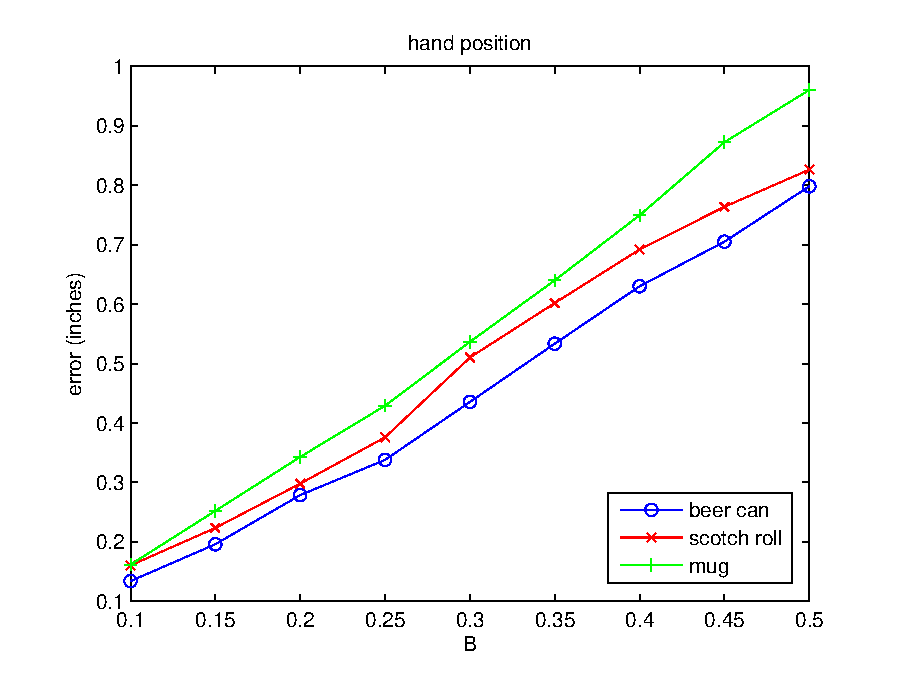
\includegraphics[width=0.32\textwidth]{error_pos.eps} &
      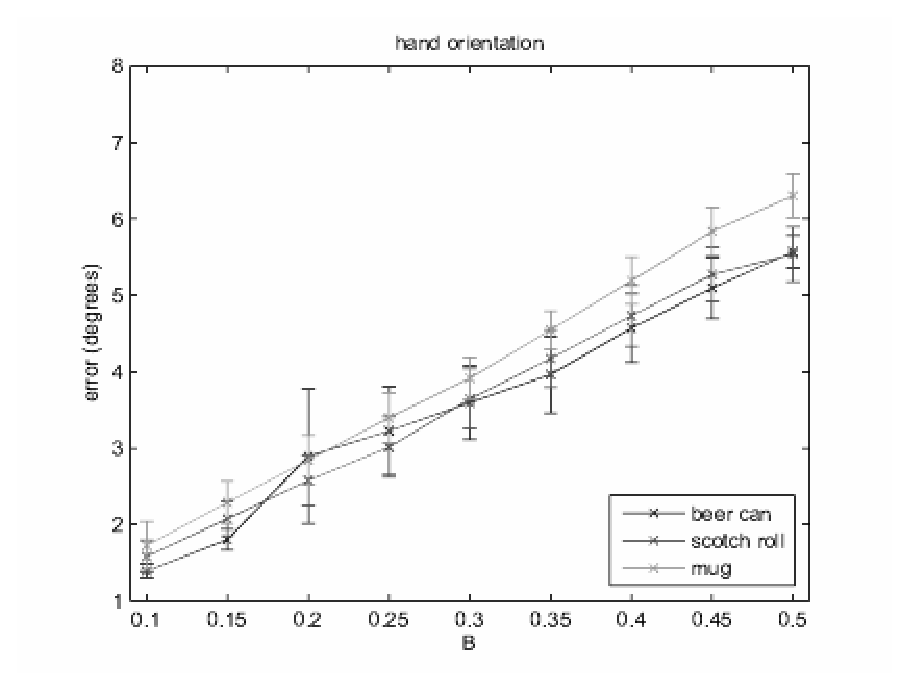
\includegraphics[width=0.32\textwidth]{error_ori.eps} &
      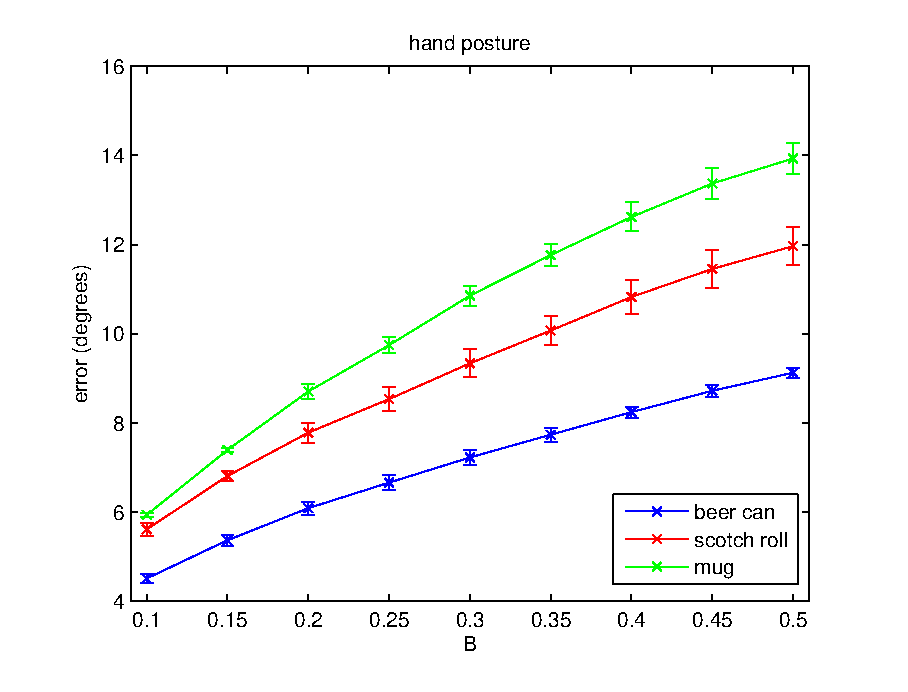
\includegraphics[width=0.32\textwidth]{error_pst.eps} \\
      $(a)$ & $(b)$ & $(c)$ \\
      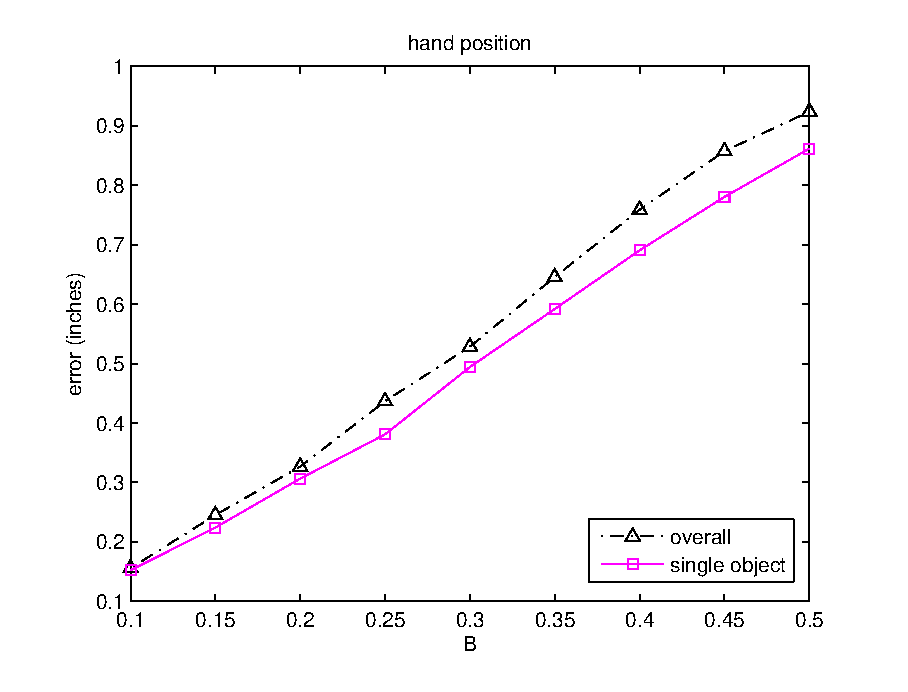
\includegraphics[width=0.32\textwidth]{error_cmp_pos.eps} &
      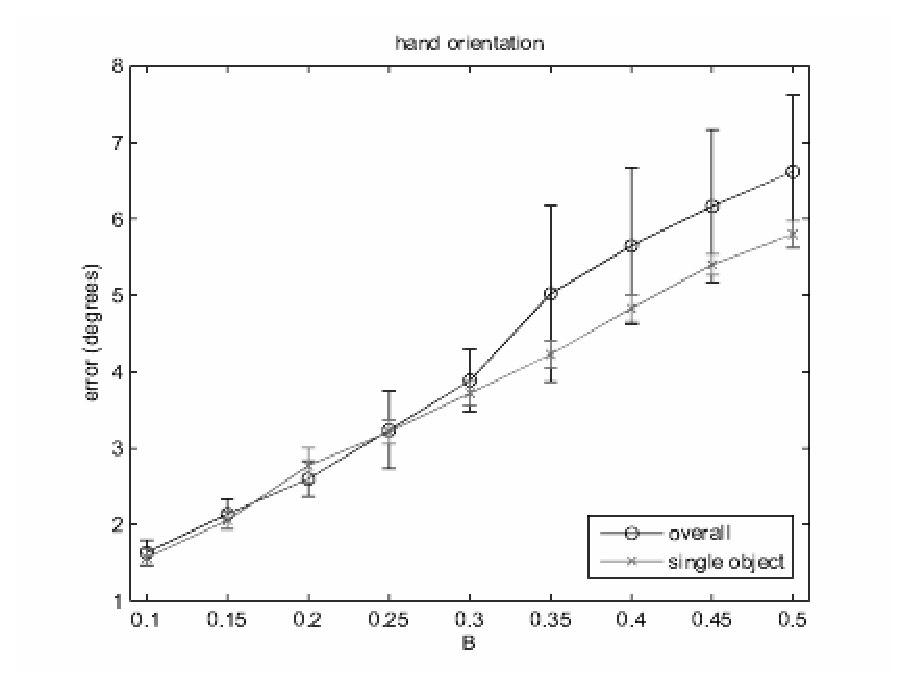
\includegraphics[width=0.32\textwidth]{error_cmp_ori.eps} &
      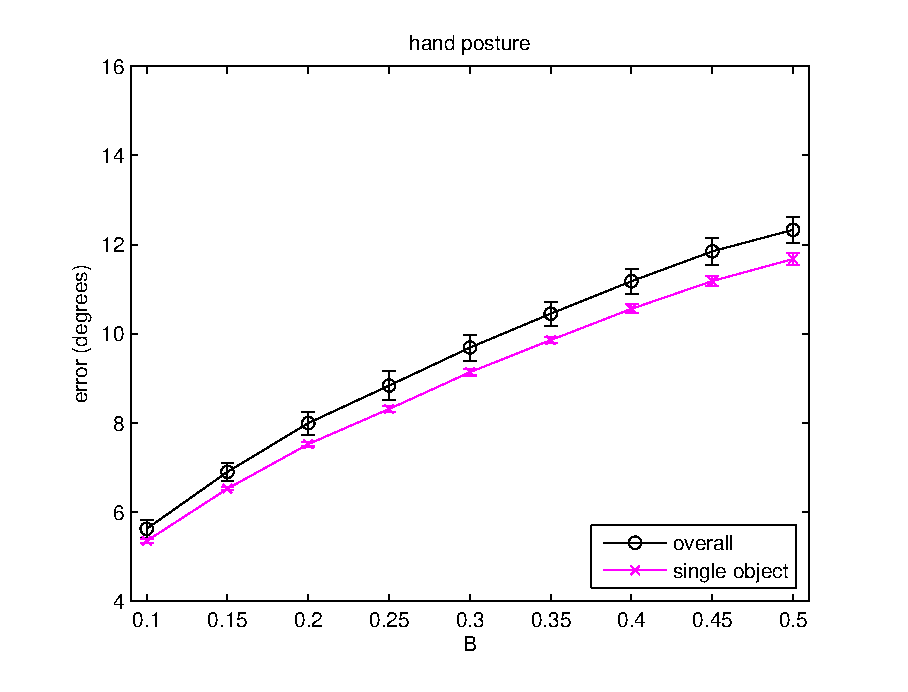
\includegraphics[width=0.32\textwidth]{error_cmp_pst.eps} \\
      $(d)$ & $(e)$ & $(f)$ \\
    \end{tabular}
    \caption{Regression results as the blind fraction $B$ increases
    from $0.1$ to $0.5$. $(a)-(c)$ comparison among the three single
    objects for the hand position, orientation and posture; $(d)-(f)$
    comparison between the average error on single objects and the
    overall error.}
    \label{fig:err_all}
  \end{center}
\end{figure}
